La idea original de la aplicación en assembler era poder procesar 16 bytes contiguos con instrucciones simultaneas para poder aprovechar al máximo el paralelismo que ofrecen las instrucciones SIMD. Esto no fué posible debido a que el set de instrucciones no tiene comparaciones de greater, lower o derivadas para bytes sin signo (necesario ya que los pixeles en grayscale van del 0 al 255) por lo que fué necesario realizar un desempaquetamiento de los datos (convirtiendolos en words) y se consiguió operar sobre los bytes de a 8 por instrucción SIMD, aunque por cada ciclo se lograron procesar los 16.

\subsubsection{Descripción del ciclo:}
Al comienzo del ciclo se ponen en 0 los bytes del registro xmm8 que servirá como acumulador de los nuevos valores que tendrán los pixeles.

Se guardan 16 bytes contiguos desde la imagen fuente en el registro xmm1, se busca cuáles son iguales al mínimo (aprovechando la instrucción pcmpeqb que realiza la comparación en los 16 bytes simultaneamente) y se guarda la máscara obtenida que se usará mas tarde. Luego se los desempaqueta en parte alta y baja extendiendolos a words para realizar comparaciones.

\begin{figure}[ht!]
\centering
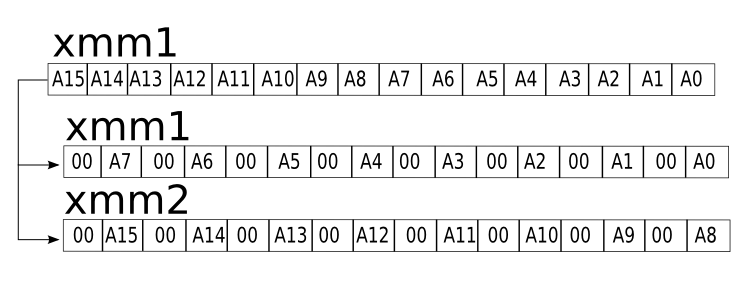
\includegraphics[width=90mm]{unpackxmm1.png}
\caption{Desempaquetado de los bytes a words para realizar comparaciones}
\label{overflow}
\end{figure}

Se buscan los números que superen al máximo comparando la parte alta y baja con el registro xmm5 preparado al inicio del programa el cuál contiene el máximo en words empaquetadas. Utilizando pcmpgtw tanto en la parte baja como la alta, obtenemos una máscara que contiene en 0xFFFF las words mayores al máximo y en 0x0000 las demás. Empaquetamos la máscara relacionada a la parte baja y a la alta dejando en 255 sólo los bytes que sean mayores al máximo para luego sumarlos en el acumulador.


\begin{figure}[ht!]
\centering
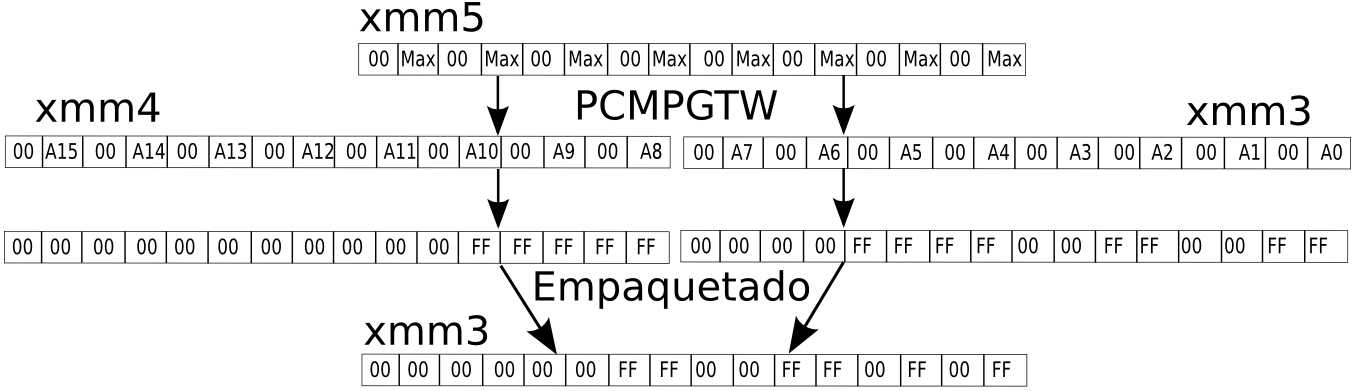
\includegraphics[width=150mm, height=40mm]{cpmmax.png}
\caption{Creación de máscara y empaquetado de la misma. El registro xmm3 es la copia de xmm1 que guardará la parte baja de la máscara, xmm4 realiza lo mismo con la parte alta.}
\label{overflow}
\end{figure}

Al utilizar un acumulador incialmente en 0 se pudo ahorrar el paso de comparar los pixeles menores al mínimo ya que los pixeles que cumplieran esta propiedad tendrían 0 como valor.

Para el caso en el que el valor del pixel estuviera entre el máximo y el mínimo ($min \geq p \leq max$) se aprovechó la máscara obtenida para los números mayores al máximo, por lo que sólo fue necesario buscar los números mayores al mínimo, agregarles los números iguales al mínimo (mediante un por) con la máscara creada al principio del ciclo y luego sacarle los mayores al máximo (mediante un pxor) con la máscara que ya se había calculado.

Luego de haber creado la máscara para el caso, se realiza el cálculo de los nuevos valores para los pixeles que cumplan esa propiedad. Fue necesario desempaquetar aún más los pixeles para poder obtener los valores de estos en double words y poder convertirlos a single precision floats, ya que esa precisión era suficiente y podría realizar más operaciones sobre los pixeles simultanteamente que con doubles.

IMAGEN
Se realiza la división por q del pixel y luego se lo convierte a entero truncandolo para realizar la función "floor" como está descripta en el enunciado. Se multiplica por q para completar el valor final del pixel y luego se vuelve a empaquetar. Se realiza la misma operación con la otra parte desempaquetada y se empaqueta otra vez para obtener el valor que cada pixel debería tener para luego aplicarle la máscara anteriormente creada y realizar una suma al acumulador que tendrá listos los valores de los bytes a mandar para luego mandarlos de a 16 bytes (double quadword).

\subsubsection{Discusión y comparación con el código C:}
Enfocandonos en la versión decompilada de umbralizar\_c.c utilizando $objdump -d -M intel -S umbralizar_c.o$ se pueden observar bien en detalle las instrucciones que utiliza el compilador para ensamblar la versión en c de umbralizar.

Se puede observar claramente que el compilador, al tratarse de el lenguaje c y su convención utiliza el stack para guardar variables locales, algo que seguramente será cubierto por la memoria caché pero que es comparable contra utilizar casi únicamente registros, que otorgan mejor performance, para almacenar datos lo cual se realiza en la implementación en assembler.

Enfocandonos un poco en los condicionales, se puede ver como la versión en c desensamblada produce el código respectivo para calcular la posición del byte específico a comparar en la matríz fuente cada vez que se quiere realizar la comparación. La eficiencia de la implementación en c es muy evidente, no sólo no es necesario calcular la posición ya que se toman 16 bytes contiguos en vez de la utilización del casteo matricial, si no que las comparaciones se realizan en simultaneo. Si bien se comparan y se procesan 8 bytes por instrucción ya que es necesario extenderlas y compararlas de a 8, en cada ciclo del algoritmo se procesan 16 bytes. Cuándo se habla de procesar, se tiene en cuenta las operaciones tanto de comparación como de cálculo para los valores resultantes de los píxeles. También queda en evidencia que el algoritmo programado en assembler hace sólo dos llamadas a memoria, una para traer los 16 bytes contiguos y otra para modificar estos 16 bytes por sus correspondientes valores, algo muy superior a pedir y modificar bytes de a uno (VER EJEMPLO TIEMPO).

Por el lado del cálculo de $floor(ecuacion) * q$ dónde $ecuacion = src_matrix[y][x] / q$ , las operaciones de punto flotante se realizan con escalares, de a una en cada iteración por el lado de c, mientras que la implementación en assembler contempla operaciones simultaneas para estas.